%%%%%%%%%%%%%%%%%%%%%%% file typeinst.tex %%%%%%%%%%%%%%%%%%%%%%%%%
%
% This is the LaTeX source for the instructions to authors using
% the LaTeX document class 'llncs.cls' for contributions to
% the Lecture Notes in Computer Sciences series.
% http://www.springer.com/lncs       Springer Heidelberg 2006/05/04
%
% It may be used as a template for your own input - copy it
% to a new file with a new name and use it as the basis
% for your article.
%
% NB: the document class 'llncs' has its own and detailed documentation, see
% ftp://ftp.springer.de/data/pubftp/pub/tex/latex/llncs/latex2e/llncsdoc.pdf
%
%%%%%%%%%%%%%%%%%%%%%%%%%%%%%%%%%%%%%%%%%%%%%%%%%%%%%%%%%%%%%%%%%%%


\documentclass[runningheads,a4paper]{llncs}

\usepackage{amssymb}
\setcounter{tocdepth}{3}
\usepackage{graphicx}
%%%%%%%%%%%%%%% New package
\usepackage{amsmath}
\usepackage{caption}
\usepackage{subfig}
\usepackage{csvsimple}
\usepackage{multirow}
\usepackage{array}
\usepackage{booktabs}
%%%%%%%%%%%%%%%
\usepackage{url}
\usepackage{float}
% \urldef{\mailsa}\path|{soltanin, locheng, ingrid.haas, frank.holzwarth,|
% \urldef{\mailsb}\path|anna.kramer, leonie.kunz, christine.reiss, nicole.sator,|
% \urldef{\mailsc}\path|erika.siebert-cole, peter.strasser, lncs}@springer.com|
% \newcommand{\keywords}\cite{1}{\par\addvspace\baselineskip
% \noindent\keywordname\enspace\ignorespaces#1}

\begin{document}

%\mainmatter  % start of an individual contribution

% first the title is needed
\title{Audio-visual speech enhancement and background noise removal}

% a short form should be given in case it is too long for the running head
%\titlerunning{Lecture Notes in Computer Science: Authors' Instructions}


% the name(s) of the author(s) follow(s) next
%
% NB: Chinese authors should write their first names(s) in front of
% their surnames. This ensures that the names appear correctly in
% the running heads and the author index.
%
\author{Han Geng\and Chen Li}
%\thanks{Please note that the LNCS Editorial assumes that all authors have used
%the western naming convention, with given names preceding surnames. This determines
%the structure of the names in the running heads and the author index.}%

%%
%\authorrunning{Lecture Notes in Computer Science: Authors' Instructions}
% (feature abused for this document to repeat the title also on left hand pages)

% the affiliations are given next; don't give your e-mail address
% unless you accept that it will be published
\institute{Group Name: Mariana}

%
% NB: a more complex sample for affiliations and the mapping to the
% corresponding authors can be found in the file "llncs.dem"
% (search for the string "\mainmatter" where a contribution starts).
% "llncs.dem" accompanies the document class "llncs.cls".
%

% \toctitle{Lecture Notes in Computer Science}
% \tocauthor{Authors' Instructions}
\maketitle


\begin{abstract}

Audio-visual speech enhancement is a coding process that suprsses the unwanted noise to highlight the useful audio signal from complex audio and video input. Recent development on video processing and audio quality enhancement provides better visual and aural experience, with the involve of deep neural network, audio/video enhancement will be improved compared to traditional method. The goal of this project is to implement a deep audio-visual speech enhancement network, which will be used to remove background noise from a given speaker video with its corresponding audio spectrogram. For research convenience, the video frames will be focused on the lip region only, and the corresponding audio clips used for both training and experiment will be a mix of the original noise-free audio signal and some generated noise signal. The program will initialize with data provided by a pre-trained network on a word-level lip-reading task, who contains labeled speaker videos and their corresponding noiseless audio signals. Our speech enhancement network will take in as input these data, where noise will be added into the audio signals, complete the training process, and then give the audio spectrum with noise removed as output. This method is different from the automatic speech recognition (ASR) who can only identify speech in a relatively noiseless environment. Instead, it can be applied to a more noisy environment where the magnitude of noise is much higher than usual (low signal-to-noise ratio), and it will also work in multi-speaker environments (such as News conference with translater's voice)
\end{abstract}


\section{Introduction}
Recent development on video processing and audio quality enhancement gives us better visual and aural experience, and the application of machine learning makes it possible for voice recognition which makes our lives even more convenient. But in the process of training and testing, the input voice signal must be recorded under relatively noiseless environment, otherwise the noise signal in the sound spectrum will cause serious deterioration in the performance, for the reason that the noise signal would add unwanted fluctuation in the spectrum and cause the spectrum to have different characteristics from its original shape, hence the machine would not recognize it as what it should be.\\
 
The major themes and applications of Automatic Speech Recognition was discussed in this paper \cite{1} in 2010, and it proposes several approaches and challenges faced by researchers in this field. For example, the context of the speech, the environment quality of the speech and the speakers themselves would influence how well the task could perform. The models proposed supports several types of speech recognition, such as isolated words, connected words, continuous speech and spontaneous speech. In order to recognize these forms of words and speech, a quiet environment must be ensured because for isolated words especially, the recognizers must obtain a test sample that does not have noise or audio signal on either side of the sample window. Imagine using Siri in a crowded station or in strong wind, it may not be able to receive exact orders that you give under such noisy environment. Maybe Siri is not a good example, but it does represent such a situation where the speech recognition system may not function as we want it to be, because of the presence of noises. Other related applications that involve outdoor or noisy activities can also be affected by low signal-to-noise ratio, such as gambling, helicopters and battleground intelligent management systems, etc.\\
 
Because of the development of speech recognition and other technical advances, people are having higher and higher demand on audio signal quality, which is often contaminated by numerous sources of natural and artificial noises. In order to improve audio quality and increase voice signal clearness, the development of voice signal enhancement and noise removal is essential.\\
 
Various graphic enhancement and noise removal techniques make it easier for us to extract useful information by recovering video or audio clips damaged by multiple source of noise, and the clearer audio signal can then be used in speech recognition and other field of applications.\\

Multiple advanced approaches to voice enhancement and noise removal have been proposed over the past few years, the most direct approach is using only audio to segregate monaural speech as supposed in \cite{2} in 2009, which is a little bit different from what we are going to propose (remove noise from single-speaker speech), but the core concept is rather similar. \cite{2} uses supervised learning techniques and computational auditory scene analysis to segregate speech recorded in one-microphone scenario. It focused mainly on the noises caused by room reverberation, which cause severe degradation to voice signal quality and is rather hard to resolve because the reverberating noise signal are mainly repetition of ground truth signal but in lower volume, hence it has similar patterns in audio spectrum as ground truth. This makes it hard for researchers to isolate just one channel of clear voice signal, and even harder when there are multiple speakers in the room, each making speeches and causing room reverberation simultaneously. Since the research only uses audio signal, the major resolution technique is to use inverse filtering, but as the paper suggested, this approach is sensitive to room condition, and the result varies for different indoor settings and reverberation conditions. They proposed a method using supervised learning approach to set up several groups for a period of time-frequency (T-F) unit, each contains a set of harmonic characteristics, then they estimate a binary mask for the time-frequency unit, and this mask filters through all the local T-F units and removes those reverberant mixtures whose target energy is weaker than the interference energy. Value 1 in the mask represents that the target is stronger than the interference, and value 0 represents the opposite.\\

\begin{figure}[h!]
%\centering
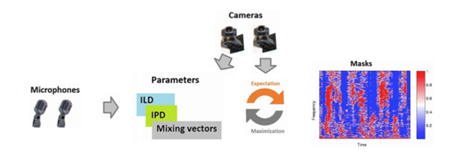
\includegraphics[scale=0.58]{fig1.png}
\caption{The direct path parameter vector is calculated with the help of video cameras. 
(The final probabilistic mask formed from the resulting probabilistic model is used for source separation)}
\label{fig:framework}
\end{figure}

As human beings when we are listening to multiple simultaneous speeches or single-speaker speech with strong noise, we are still able to distinguish the target speaker that we want to hear from other unwanted interfering noises. One reason being that we are using two ears for audio input which gives more characterizing information about the target speaker, but the most helpful and obvious devices that we use to distinguish target speaker is through our eyes.\\
 
Since we can observe visual information about our surroundings, we know when the speaker is talking when we see their mouths moving, and from this we know precisely which part of audio clips contains the speech that we desire, and everything happening outside the range of mouth movement is considered noises automatically. With the help of the video information, we can even generate audio signals from a silent video clip if we have trained a model to identify mouth movement and match it to words and sentences as discussed in \cite{3}, but this is beyond the scope of the topic of interest. Nevertheless, we can reduce the workload by a great amount and focus on removing noises from only part of the whole audio samples that contains the target speaker’s speech, if we have the visual information about the speaker and align it chronologically with the audio samples. The use of corresponding video signals as reference for speaker separation is proposed in \cite{4}. This paper focused on separating single-channeled speakers with help of corresponding visual information.\\
 
They record simultaneous speeches given by multiple speakers through a single-channel microphone, and capture videos of these speakers when they are giving the speeches. Using similar techniques as described above, they create a T-F binary mask generated from the visual information that defines which part of the audio is corresponding to the speaker video clip, then filter through the audio signals to retain the dominant speech signals. In this binary mask, value of 1 means the target speaker is talking, and 0 means the speaker is not talking and thus T-F unit is masked. The point of this method is to estimate which part of the T-F component and frequency unit should be retained.\\

\begin{figure}[h!]
%\centering
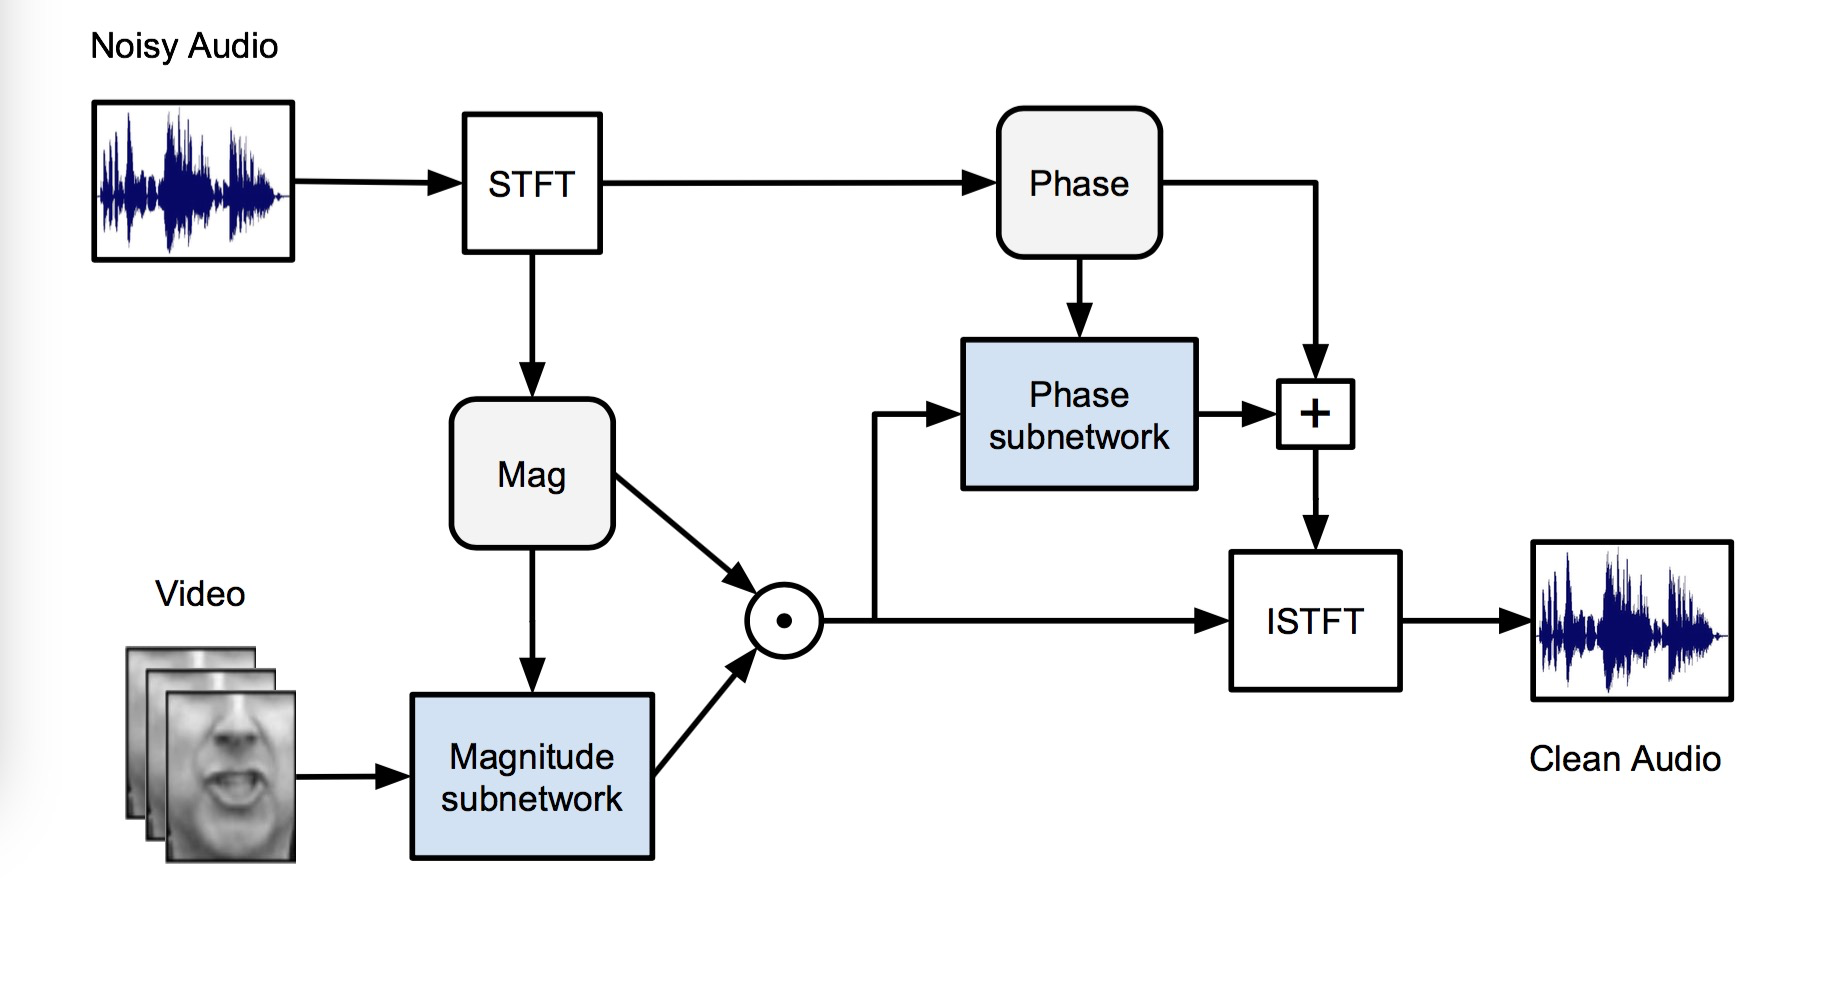
\includegraphics[scale=0.19]{fig3.png}
\caption{Audio-visual speech enhancement architecture}
\label{fig:framework}
\end{figure}

This method requires training of a generalized method of moments (GMM) to model audio and visual speech features, so that the correspondence between the audio and visual features can be used to estimate the audio features from the given videos, since this correspondence has been proposed to be valid by several studies in \cite{5} and \cite{6}.\\

%%% 11-8 12-9 13-10 14-11 15-12 16-13
In 2017, A. Gabbay et, al. \cite{8} Implemented a model that can extract a specific visible speaker’s voice from the similar background noise environments using video data and audio spectrograms. In their study, for unconstrained environments, the separation of the specific speaker requires (i) a sequence of video frames showing the mouth of the speaker; and (ii) a spectrogram of the noisy audio. The source of the audio and video then went through encoder respectively then embedded into fc-layers. Encoding module is composed of a dual tower Convolutional Neural Network in order to make the input from audio/video source have the same embedded representing feature. The video encoder and the audio encoder functions different roles. The video encoder crops from the center of the mouth region of the frames then feed the consecutive gray-scaled cropped frames to consecutive convolution layers (note the layers using Batch Normalization \cite{9} and Leaky-ReLU \cite{10} mathematic matrix processing to filter the frames). The audio encoder receives the input audio spectrogram clips correspond to the video frames fed into the video encoder. The audio encoder also uses convolution layers with Batch Normalization \cite{9} and Leaky-ReLU \cite{10} to filter the audio clips. Both encoders result in the feature vector with the same embedding as output. The two encoders output shared representation to consecutive fully-connected layers. An audio decoder is accepting the data passed through consecutive fully-connected layers with transposed convolution layers to represent the enhanced speech.\\

\begin{figure}[H]
%\centering
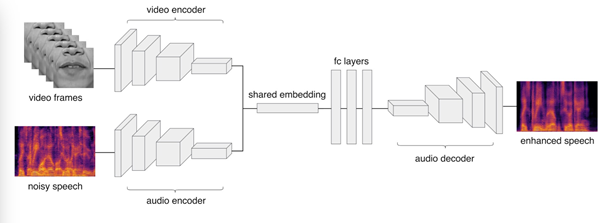
\includegraphics[scale=0.60]{fig4.png}
\caption{Audio/video encoder and decoder model for the study below}
\label{fig:framework}
\end{figure}
 
Aside from the model with video and magnitude of the audio signal example above, \cite{11} in 2017, J.-C. Hou et, al. Introduced a voice enhancement model based on neural network training from a variety of noise features that is able to enhance specific speaker’s voice pattern from different kinds of noise backgrounds. The model incorporates audio and visual streams into a unified network model \cite{12}. Using AVDCNN as the audio-visual encoder-decoder network to perform the voice enhancing job. Where AVDCNN is for Audio-Visual Deep Convolutional Neural Network. Similar to the model introduced by A. Gabbay et al., the model introduced by J.-C. Hou et, al. processes audio and visual streams using two independent convolutional neural networks. A fusion network is following the two convolutional neural networks to fuse them together with maximum pooling layer and fully-connected layer \cite{11}.
This model uses back-propagation to jointly learn the parameters in an end-to-end manner \cite{12}.\\

\begin{figure}[H]
%\centering
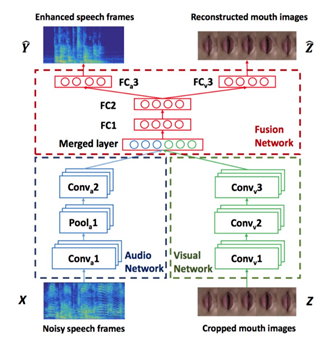
\includegraphics[scale=0.38]{fig5.png}
\caption{Construction of the AVDCNN model for the study above}
\label{fig:framework}
\end{figure}

\section{Data Set}
In order to generate a model for speech recognition and noise removal, we need a large dataset for training and testing the model, one suitable option is VoxCeleb2, which is also used in \cite{7}. It is an open-source media that contains huge amount of audio-visual speaker recognition dataset that we can use in our convolutional neural network training process, which will be discussed in later section. The study proposed in \cite{7} presents a deep CNN based neural speaker embedding system called VGGVox, which is trained to project the voice signal spectrum to Euclidean space, where the Euclidean distance represent the similarity of speakers.\\

\begin{figure}[H]
%\centering
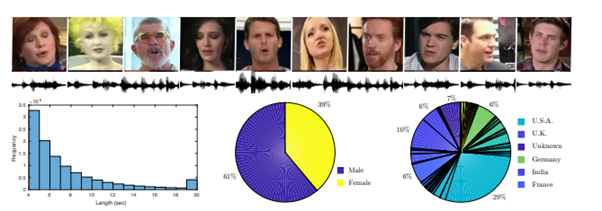
\includegraphics[scale=0.6]{figure3.png}
\caption{Top row: Examples of faces from the VoxCeleb2 dataset.\\Bottom row: (left) distribution of utterance lengths in the dataset – length shorter than 20s are binned in 1s intervals and all utterances of 20s+ are binned together; \\(middle) gender distribution and (right) nationality distribution of speakers. \cite{7}}
\label{fig:framework}
\end{figure}



%%% add words %%%


\section{Proposed Method}
The algorithm requires audio signal with diversity aspect of noise interacted with the original speaker voice.\\
In order to create original speaker voice with different kinds of noise mixure we used pysndfx package \cite{19} to add different kinds of noise to the given '.wav' file. \\
The pysndfx package applies audio effects such as reverb and EQ directly to audio files or NumPy ndarrays. The pysndfx package is a lightweight Python wrapper for SoX - Sound eXchange. Where Sox is a cross-platform command line utility that can convert various formats of computer audio files in to other formats. It can also apply various effects to these sound files, and SoX can play and record audio files on most platforms. \cite{20} The pysndfx supports effects range from EQ and compression to phasers, reverb and pitch shifters. Before importing the pysndfx package the terminal should be installed the package related application. (using pip command to install the package related application)\\

We added mixured level of highshelf, lowshelf filters and reverb, phaser, delay effects to the oriaginal sound and outputed the prcessed sound file and comparsion spectrogram.\\

A low shelf will either cut or boost signals below a c.o.f. in a manner resembling a shelf, or an equal strength amplitude band past the rolloff. A high shelf filter will either cut or boost signals above a c.o.f. similarly.
Where c.o.f stands for cutoff frequency at the point a specific frequency component would have lost approximately half the power (-3 dB) of unaffected frequencies, often referred to as the half-power point. A common synthesis technique is to sweep the cutoff frequency up or down to provide a 'spectral shape' to a sound over time. Cutoff frequencies are usually controlled by an envelope generator or an oscillator (timbre modulation).\cite{21}\\
%HLshelf.jpeg

\begin{figure}[H]
%\centering
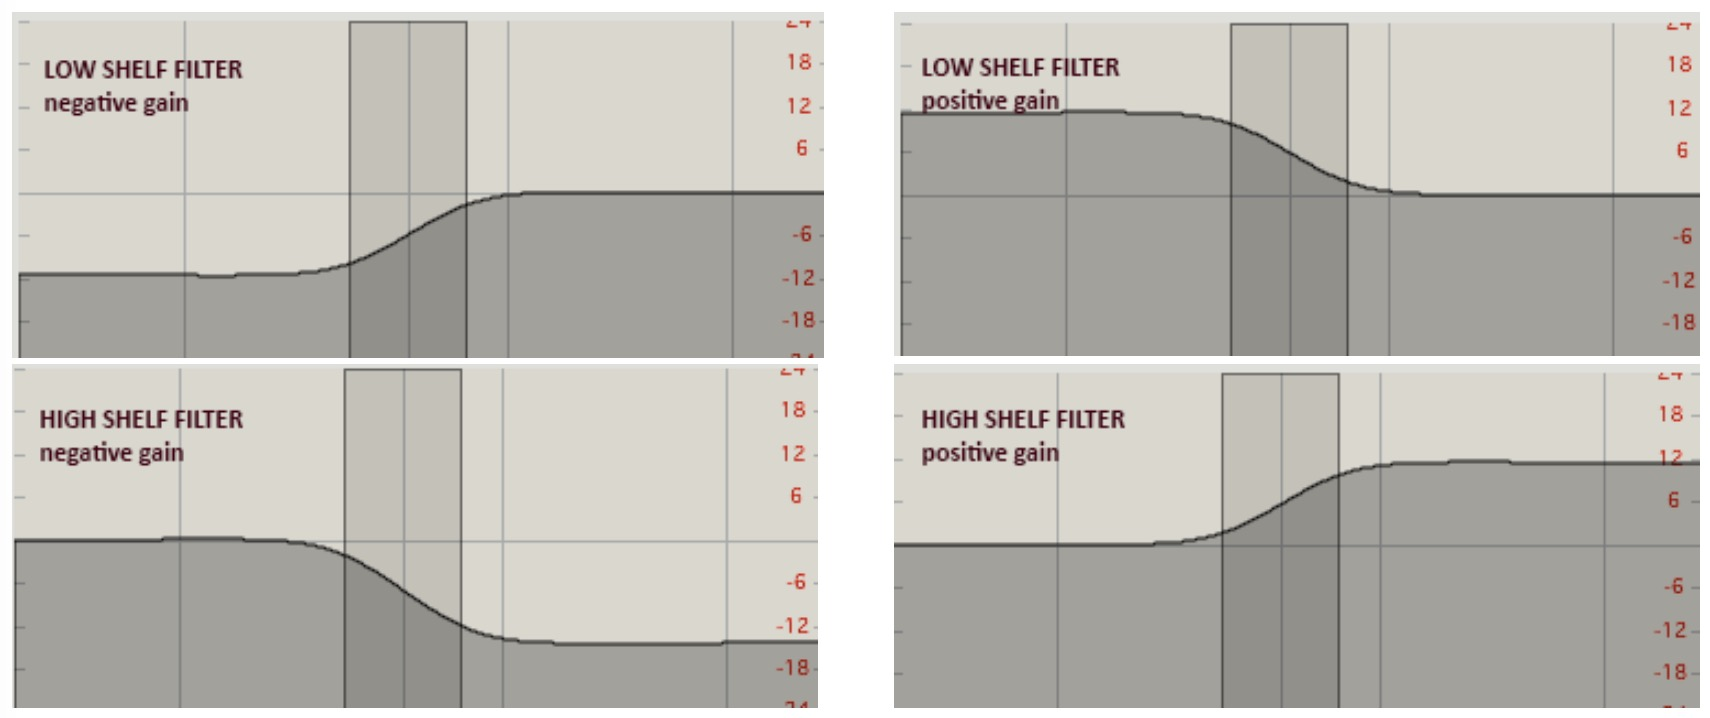
\includegraphics[scale=0.15]{HLshelf.jpeg}
\caption{Shelf transfer function \cite{21}}
\label{fig:framework}
\end{figure}


In detail, The analog transfer function for a low shelf is:\\
%%high_shelf_formula.png%%	\cite{22}
\begin{figure}[H]
%\centering
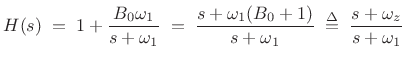
\includegraphics[scale=0.60]{high_shelf_formula.png}
\caption{Low shelf transfer function \cite{22}}
\label{fig:framework}
\end{figure}

where $B_0$ is the dc boost amount (at s = 0), and the high-frequency gain (s = ∞) is constrained to be 1 . The transition frequency dividing low and high frequency regions is w1 . See Appendix E for a development of s-plane analysis of analog (continuous-time) filters. \cite{23}\\
A high shelf is obtained from a low shelf by the conformal mapping (s <-- 1/s) , which interchanges high and low frequencies.\\
%%high_shelf_formula2.png%%  \cite{22}
\begin{figure}[H]
%\centering
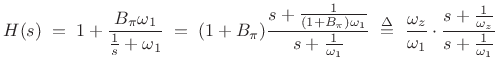
\includegraphics[scale=0.60]{high_shelf_formula2.png}
\caption{High shelf transfer function \cite{22}}
\label{fig:framework}
\end{figure}

In this case, the dc gain is 1 and the high-frequency gain approaches.\\
%%shelf_formula3%%
\begin{figure}[H]
%\centering
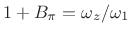
\includegraphics[scale=0.60]{shelf_formula3.png}
%\caption{High shelf transfer function \cite{22}}
\label{fig:framework}
\end{figure}

Low and high shelf filters are typically implemented in series, and are typically used to give a little boost or cut at the extreme low or high end (of the spectrum), respectively. To provide a boost or cut near other frequencies, it is necessary to go to (at least) a second-order section, often called a peaking equalizer. \cite{23}\\























%%%%%%% That's sara's stuff below %%%%%%%%%%%
%\begin{table}[h]\small
%  \centering
%  \caption{Demographics of the PPMI}
%  \begin{tabular}{|>{\bfseries}c|*{7}{c|}}\hline
%    \multirow{2}{*}{\bfseries Data Type}
%    & \multicolumn{2}{c|}{\bfseries Class}
%    &\multicolumn{2}{c|}{\bfseries Sex}
%    & \multicolumn{3}{c|}{\bfseries Age} \\\cline{2-8}
%    & \textbf{PD} & \textbf{HC} & \textbf{F}&\textbf{M} & \textbf{(25-50)}&\textbf{(50-76)} &\textbf{(75-100)}\\ \hline
%           Number of Subjects   &411 & 187 & 217 & 381 & 81&472&45      \\ \hline
%  \end{tabular}
%  \label{tab:ppmi}
%\end{table}

The overview of our proposed method is presented in Fig.\ref{fig:framework}  which has $3$ general steps including: 1- Preprocessing; 2- Feature Extraction; and 3- Classification. Next, each step is explained in detail. The goals of CAD system goals are:
\begin{enumerate}
\item Extracting the volume based features from the MR T1 images using the automated surface-based analysis package FreeSurfer.
\item Comparing the capability of different types of classifiers for diagnosing PD.
\end{enumerate}

\begin{figure}[h!]
%\centering
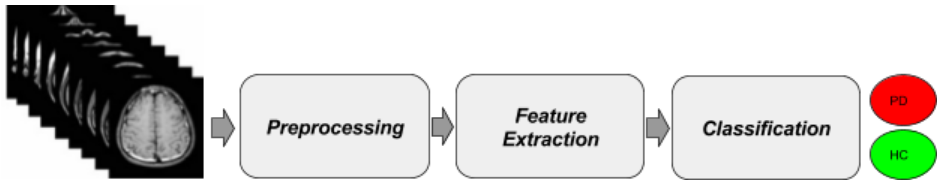
\includegraphics[scale=0.37]{flchart.png}
\caption{The general framework of the proposed methods.}
\label{fig:framework}
\end{figure}
\subsection{Preprocessing}
Preprocessing is an essential step in designing the CAD system which provides informative data for the next steps. In this paper, for computing the volumetric information of the MRI subject’s, several preprocessing steps are needed. The Freesurfer image analysis suite is used for performing preprocessing over the 3D MRI data. FreeSurfer is a software package for the analysis and visualization of structural and functional neuroimaging data from cross-sectional or longitudinal studies \cite{16}. The FreeSurfer pipeline performs cortical reconstruction and subcortical volumetric segmentation including the removal of non-brain tissue (skull, eyeballs and skin), using an automated algorithm with the ability to successfully segment the whole brain without any user intervention \cite{f}. FreeSurfer is the structural MRI analysis software of choice for the Human Connectome Project which is documented and freely available for download on-line (http://surfer.nmr.mgh.harvard.edu/). In total 31 preprocessing steps has completed using FreeSurfer, of which some are shown in Fig.\ref{fig:prepsteps}.
\begin{figure}
\centering
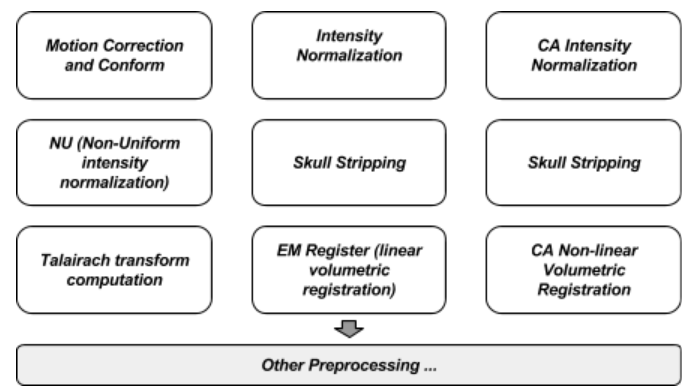
\includegraphics[scale=0.4]{Preprocessing.png}
\caption{Preprocessing steps.}
\label{fig:prepsteps}
\end{figure}

There are two types of failures in the preprocessing step which can be categorized into hard failure and soft failure. Hard failures are related to the subjects for whom preprocessing is not successful and the soft failure are related to the subjects that are preprocessed but there are some problem in the results of preprocessing. Out of $568$ subjects MRIs, $388$ images were successfully preprocessed. Other images were excluded from
the dataset due to poor quality of the original images
or unknown CDR labels.

\subsection{Feature Extraction}
After preprocessing using FreeSurfer, a list of volume based features are extracted from different regions of the brain. These features are captured from the regions segmented by brain parcellation using FreeSurfer. Some of the features collected in the left and right hemispheres of the brain are listed below:
\begin{enumerate}
	\item Left and right lateral ventricle
	\item Left and right cerebellum white matter
	\item Cerebrospinal fluid (CSF)
	\item Left and right hippocampus
	\item left and right hemisphere cortex
	\item Estimated total intra cranial (eTIV)
	\item left and right hemisphere surface holes
\end{enumerate}
The extracted feature data is based on Equation \ref{eq:fd}.
\begin{equation}
FeatureData =
\begin{bmatrix}
    f_{11}       & f_{12} & f_{13} & \dots & f_{1n} \\
    f_{21}       & x_{22} & x_{23} & \dots & f_{2n} \\
    %\hdotsfor{5} \\
    \qquad \ldots\\
    f_{s1}       & f_{s2} & f_{s3} & \dots & f_{sn}
\end{bmatrix}
%FeatureData = [f_{i,j}] \quad i \in [1:n], j\in [1:m]\\
\label{eq:fd}
\end{equation}
Where $s$ is the number of subjects and $n$ is the number of extracted features for that subject. In this study, $n$ is $388$ and $m$ is $139$.

Furthermore, there are two other type of features which are provided by the PPMI dataset which are age and sex for each subject. Thus, these two biographical information could be added to the extracted feature which gives feature data with the size $(388*141)$.
\subsection{Classification}
In this part the aim is using the extracted volume based features for classifying the MRI data into two classes of PD and HC. In our study, three types of supervised classification algorithm are used. Next, each classification method is described:
\begin{itemize}
\item \textbf{Logistic Regression (LR):}\\
Logistic regression (LR) is a statistical technique which is used in machine learning for binary classification problems. LR belongs to the family of MaxEnt classifiers known as the exponential or log-linear classifiers \cite{LR}. Like naive Bayes, it works by extracting some set of weighted features from the input, taking logs, and combining them linearly (meaning that each feature is multiplied by a weight and then added up) \cite{17}. Thus, this model is a suitable binary classifier for our problem.
\item \textbf{Random Forest (RF):}\\
Random forests (RF) is an ensemble learning method for classification, regression and other tasks. This method is presented by Breiman \cite{18}, which creates a set of decision trees from a randomly selected subset of training data. It then aggregates the votes from different decision trees to define final class of the test object. Each tree in a random forest is a weak classifier. A large set of trees trained with randomly chosen data makes a single decision on a majority basis. In the current stage of this research, we tested how accurate decisions can be made by random forests trained by the data coming from a single MRI volume.
\item \textbf{Support Vector machine (SVM):} \\
Support vector machine (SVM) \cite{19} is a well-known supervised machine learning algorithm for classification and regression. It performs classification tasks by constructing optimal hyperplanes in a multidimensional space that separates cases of different class labels. This classification method is more popular because it is easier to use, has higher generalization performance and less tuning comparing to other classifiers. In our case, the kernel SVM is used.

\end{itemize}

There is a set of parameters for each classifier that needs to be tuned in order to have a fair comparison.

\section{Results and Discussion}
In this section, the experimental results for different steps of the proposed CAD system for diagnosis of PD is presented. First the preprocessing step prepares the MRI data for the next steps using FreeSurfer. Fig.\ref{fig:prepres} shows the MRI for subject $3102$ and the resulting image after preprocessing.

\begin{figure}[!h]\small
  \centering
  \subfloat[Original MR image.]{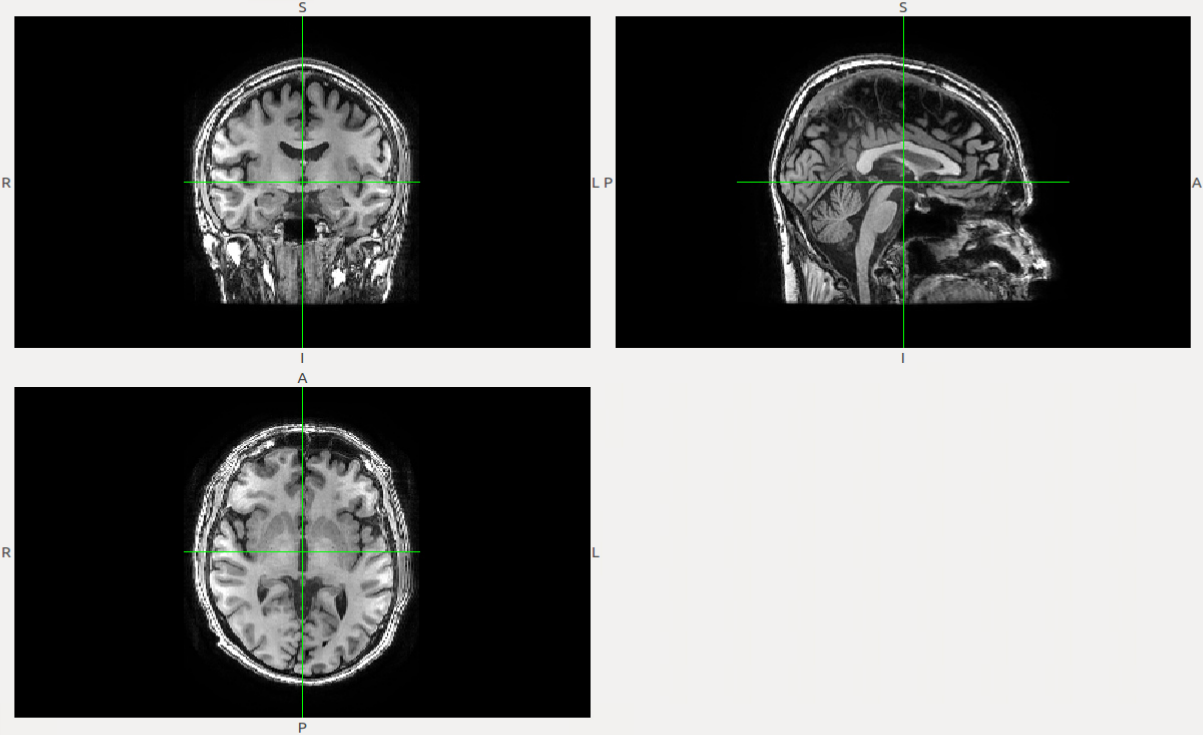
\includegraphics[scale=0.25]{orgimg.png}\label{fig:f1}}%[width=0.5\textwidth]
  \hfill
  \subfloat[Preprocessed MR image.]{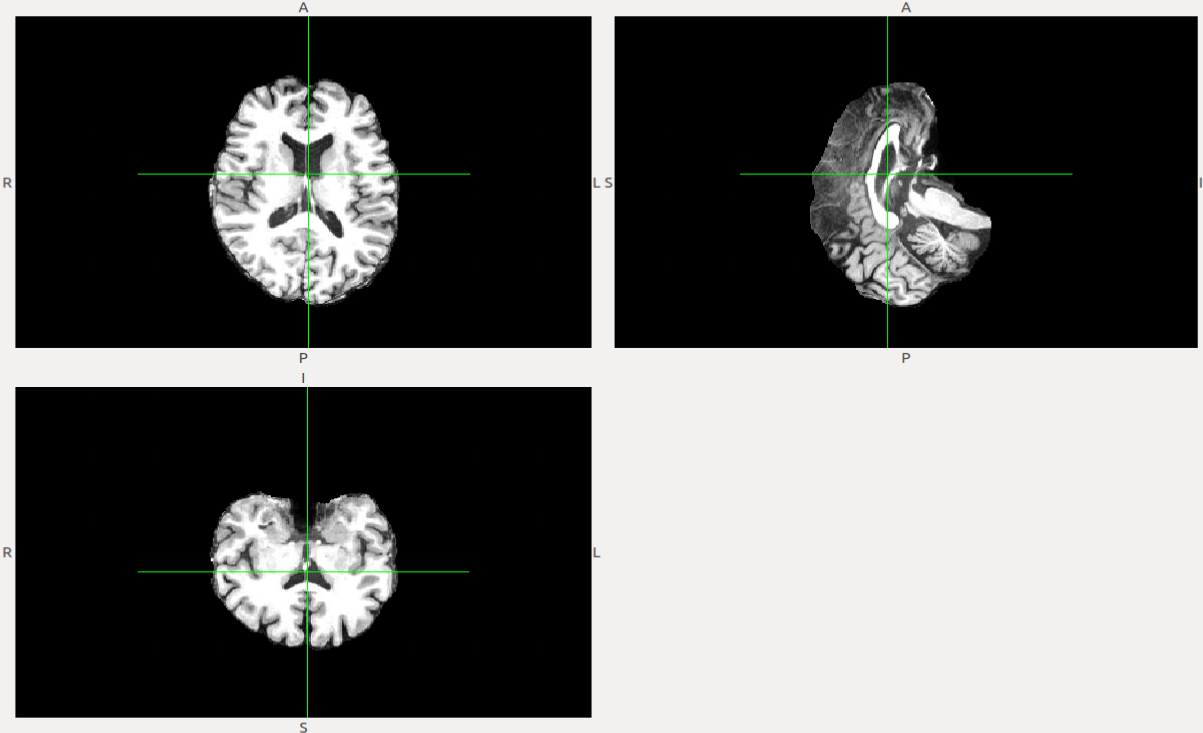
\includegraphics[scale=0.25]{prep.png}\label{fig:f2}}
  \caption{Preprocessing results for one of the subjects.}
  \label{fig:prepres}
\end{figure}
After preprocessing with FreeSurfer, for each subject a list of volume-based features is extracted. Also, age and sex are provided for the PPMI data in their website as demographic information of the patients. Some evaluation has been done over the set of extracted features in terms of their discrimination ability. Since PD is an age related disease, the distribution of data in terms of age feature is plotted. Fig.\ref{fig:agelabel} shows the distribution of age in the dataset for the subjects with PD and HC labels.
\begin{figure}[h]\small
\centering
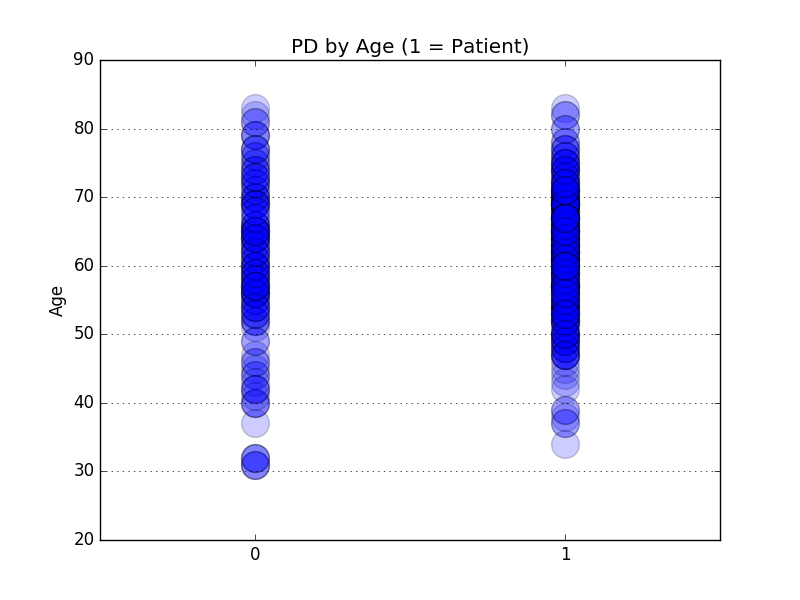
\includegraphics[scale=0.4]{AgeData.png}
\caption{Distribution of Data in terms of Age feature.}
\label{fig:agelabel}
\end{figure}
The distribution of all the extracted features are plotted in terms of their ability to distinguish the data into two classes of PD and HC. Some of these distributions are shown in Fig.\ref{fig:feateval}. As can be seen in Fig.\ref{fig:feateval}(a), the subjects with PD have higher brain volume compared to healthy ones. Furthermore, the distribution in Fig.\ref{fig:feateval}(b) and (c) illustrate that when people are in the PD category, their CSF and their CC-Anterior  volume size is enlarged. Fig.\ref{fig:feateval}(d) shows that the surface hole volume in PD is noticeably higher than the normal subjects.
\begin{figure}[h]\small
  \centering
  \subfloat[]{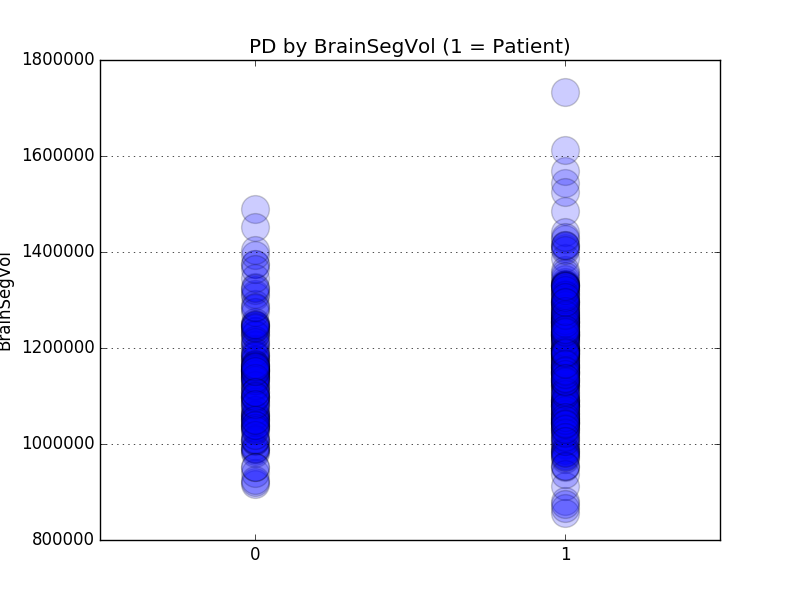
\includegraphics[width=0.5\textwidth]{Parkinson-distribution-BrainSegVol.png}\label{fig:f1}}
  \hfill
  \subfloat[]{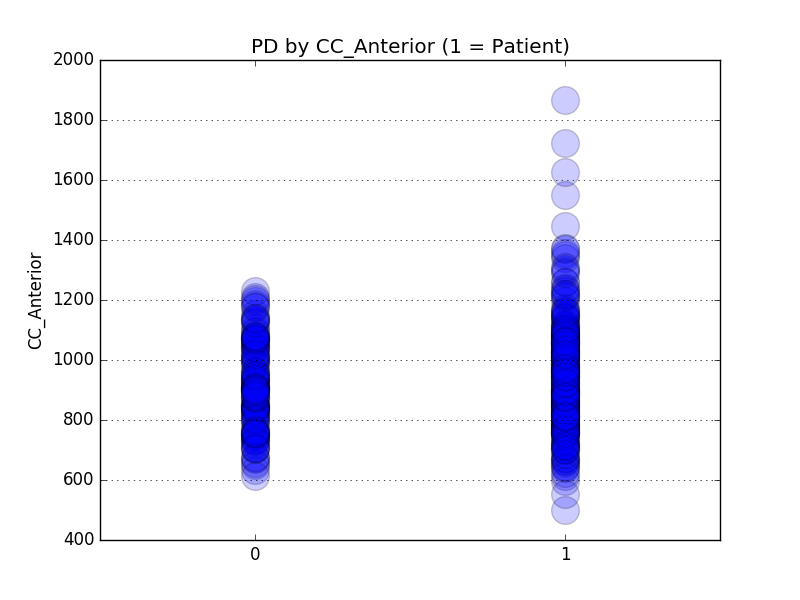
\includegraphics[width=0.5\textwidth]{Parkinson-distribution-CC_Anterior.png}\label{fig:f2}}
  \\
    \subfloat[]{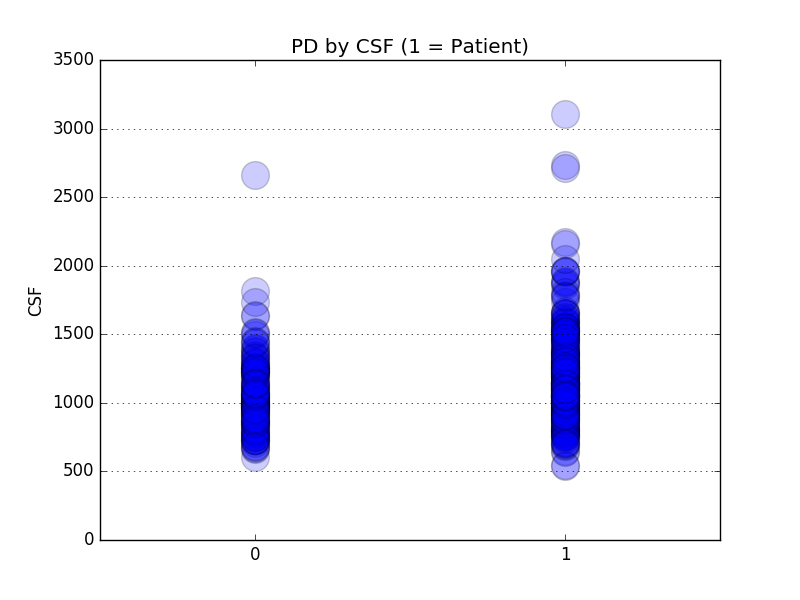
\includegraphics[width=0.5\textwidth]{Parkinson-distribution-CSF.png}\label{fig:f1}}
  \hfill
  \subfloat[]{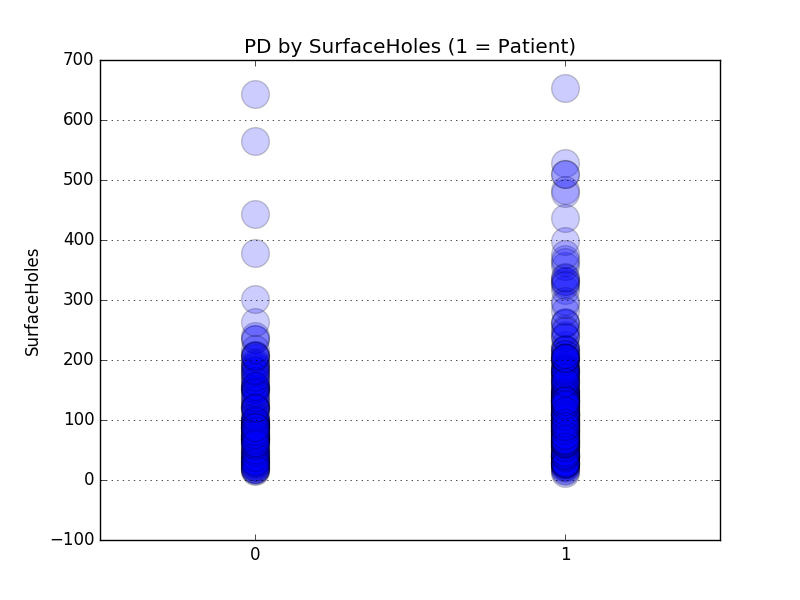
\includegraphics[width=0.5\textwidth]{Parkinson-distribution-SurfaceHoles.png}\label{fig:f2}}
  \caption{Data distributions in terms of the class labels and corresponding features; which are: (a) Brain segmented volume. (b) CC- Anterior. (c) CSF. (d) Surface holes.}\setlength{\belowcaptionskip}{0pt}
  \label{fig:feateval}
\end{figure}
Another set of evaluation is done over the extracted features. Data for every two features are plotted versus each other based on the corresponding class. Fig.\ref{fig:pairfeat} shows the distribution of data based on the two pair of features including $3rd$ ventricles vs lateral ventricles and $3rd$ ventricles vs. left vessels. In both of them, two features tend to have bigger value when the subject is PD.

\begin{figure}[!tbp]
  \centering
  \subfloat[]{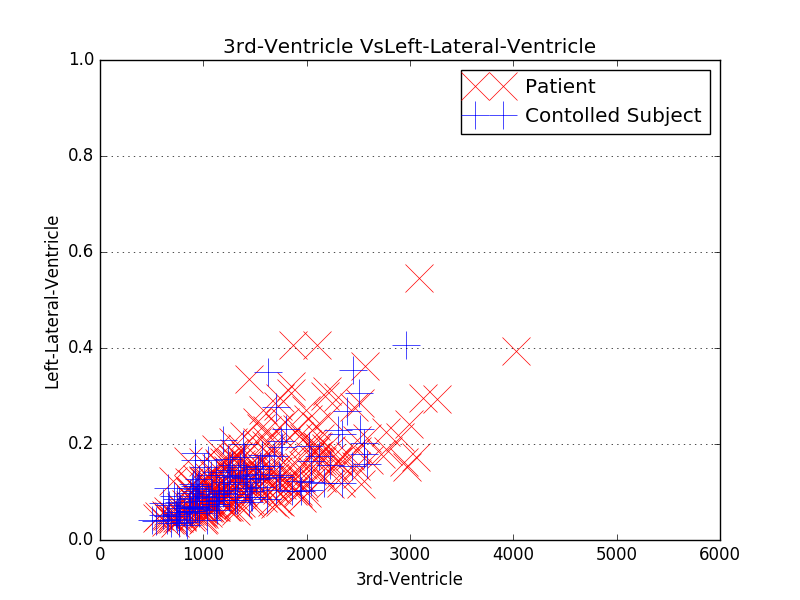
\includegraphics[width=0.5\textwidth]{3rd-Ventricle-Left-Lateral-Ventricle.png}\label{fig:f1}}
  \hfill
  \subfloat[]{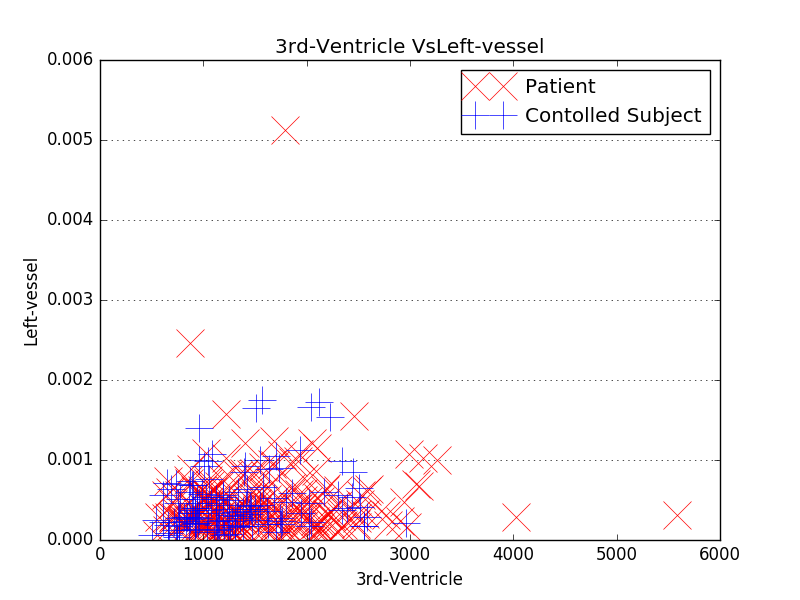
\includegraphics[width=0.5\textwidth]{3rd-Ventricle-Left-vessel.png}\label{fig:f2}}
  \caption{Data distribution based on the pair of features: (a)3rd ventricle and left lateral ventricle. (b) 3rd ventricle and left vessel.}
  \label{fig:pairfeat}
\end{figure}
As explained in the previous section, three types of classifiers are used in this study. These algorithm are run over $388$ samples with $141$ features. Internal and external cross validation is applied with $K=10$ for external and $k=5$ for internal (parameter tunning cross validation). The number of selected samples for the training part is $350$ and for the test part is $38$. Furthermore, the number of PD and HC in each group is presented in Table \ref{tab:trtedata}.
\begin{table}[h]\small
\centering
\caption{Data balance in training and testing parts.}\setlength{\abovecaptionskip}{0pt}
\begin{tabular}{|c|c|c|c|}
\hline
         & PD  & Hc  & Total \\ \hline
Training & 236 & 114 & 350   \\ \hline
Test     & 26  & 12  & 38    \\ \hline
\end{tabular}
\label{tab:trtedata}
\end{table}

As mentioned before, the classification algorithm needs a set of parameters for tunning which is selected as follow:
\begin{itemize}
\item logistic Regression (LR):\\
Regularization = $[1e-1, 1e-2, 1e-3, 1e-4, 1e-5]$, Tolerance = [1e-1, 1e-2, 1e-3, 1e-4, 1e-5]
\item Random Forest (RF):\\
Number of estimator =$[5, 10, 15, 20, 25]$, Max depth = $[2-10]$
\item Support Vector Machine (SVM): \\
C = $[0.1, 1, 10, 100, 1000]$, Gamma = $[10, 1, 1e-1, 1e-2, 1e-3, 1e-4]$, kernels = $[linear, rbf, poly]$
\end{itemize}
The evaluation metrics used in this paper for comparing the results of the classification algorithms include accuracy, confusion matrix (recall, precision) and AUC (area under ROC curve). The classification results for LR, RF and SVM are shown in Tables \ref{tab:logit}, \ref{tab:rf}, and \ref{tab:svm}, respectively.

\begin{table*}[h]\small
	\centering
	\caption{Logistic regression performance}
	\label{tab:logit}
	\csvautotabular{Logistic.csv}
\end{table*}

\begin{table*}[h]\small
	\centering
	\caption{Random forests performance}
	\label{tab:rf}
	\csvautotabular{RF.csv}
\end{table*}

\begin{table*}[h]\small
	\centering
	\caption{Support Vector Machine performance}
	\label{tab:svm}
	\csvautotabular{SVM.csv}
\end{table*}
Table \ref{tab:comp} shows the general comparison between these methods. The best result is for RF. In the table there are two sets of results related to using age/sex feature or doing the classification based only on the extracted volume based features from FreeSurfer.

Based on the literature review, most papers use VBM for data analysis and feature extraction. In this paper, one of the important goals was evaluating the FreeSurfer features for PD MRIs using machine learning techniques.  Generally, the experimental results show that the classification models need more information about the data that should be added to the current features, since these are low-level features and we need a set of high-level features as well. In future research, we are going to determine the useful general features that can be combined with the volume based extracted features.
\begin{table*}[h]\small
	\centering
	\caption{Comparing performance of different classifiers}
	\label{tab:comp}
	\csvautotabular{compmet.csv}
\end{table*}
\section{Conclusion}
We presented an automatic MRI based CAD system for diagnosing Parkinson’s Disease (PD) which is the second common neurodegenerative disease affecting elderly people. This disease is exposed by loss of neuro-transmitters that control body movements and there is no cure other than earlier diagnosis with better and more efficient treatment for patients. MR T1 images from the public PPMI PD data set is used. FreeSurfer is used for feature extraction and preprocessing. The decision model for classification of the extracted feature data is based on LR, RF and SVM methods. In the experimental results, the ability of these three types of classifiers for PD diagnosis are compared to each other. Results show that using only MRI is a potential option for PD diagnosis. This approach will avoid exposing the brain to harmful radiation based scans. In future work, the efficiency of the proposed method could be improved by adding high level features to the current ones. The classification rate with MRI needs to be improved to get close to those using raditation based scanning.
\begin{thebibliography}{4}

\bibitem{1} M. Anusuya and S. K. Katti, “Speech recognition by machine, a review,” arXiv preprint arXiv:1001.2267, 2010.


\bibitem{2} Z.Jinand D.Wang,“A supervised learning approach to monaural segregation of reverberant speech,” IEEE Transactions on Audio, Speech, and Language Processing, 2009.


\bibitem{3}  A. Ephrat, T. Halperin, and S. Peleg, “Improved speech reconstruction from silent video,” in ICCV 2017 Workshop on Computer Vision for Audio-Visual Media, 2017.


\bibitem{4} F.KhanandB.Milner,“Speaker separation using visually-derived binary masks,” in AVSP, 2013


\bibitem{5}  H. Yehia, P. Rubin, and E. Vatikiotis-Bateson, “Quantitative association of vocal tract and facial behavior,” Speech Communication, vol. 26, no. 1, pp. 23–43, Oct. 1998.


\bibitem{6} I. Almajai and B. Milner, “Visually-derived Wiener filters for speech enhancement,” IEEE Trans. Audio, Speech and Language Processing, vol. 19, no. 6, pp. 1642–1651, Aug. 2011.


\bibitem{7} J. S. Chung, A. Nagrani, , and A. Zisserman, “VoxCeleb2: Deep speaker recognition,” arXiv preprint arXiv:1001.2267, 2018.


\bibitem{8} A. Gabbay, A. Shamir, and S. Peleg, “Visual Speech Enhancement using Noise-Invariant Training,” arXiv preprint arXiv:1711.08789, 2017.


\bibitem{9} S. Ioffe and C. Szegedy. Batch normalization: Accelerating deep network training by reducing internal covariate shift. In ICML’ 15, pages 448–456, 2015.


\bibitem{10} A.L.Maas,A.Y.Hannun,andA.Y.Ng.Rectifier nonlinearities improve neural network acoustic models. In ICML’ 13, volume 30, 2013.


\bibitem{11} J.-C. Hou, S.-S. Wang, Y.-H. Lai, Y. Tsao, H.-W. Chang, and H.-M. Wang, “Audio-Visual Speech Enhancement Using Multi- modal Deep Convolutional Neural Networks,” IEEE Transactions on Emerging Topics in Computational Intelligence, 2018.


\bibitem{12} J.-C. Hou, S.-S. Wang, Y.-H. Lai, J.-C. Lin, Y. Tsao, H.-W. Chang, and H.-M. Wang. Audio-visual speech enhancement based on multimodal deep convolutional neural network. arXiv:1703.10893, 2017.
%%% 11-8 12-9 13-10 14-11 15-12

\bibitem{13} 

\bibitem{14} 

\bibitem{15} 

\bibitem{16} 

\bibitem{f}  

\bibitem{LR} 

\bibitem{17} 

\bibitem{18} 

\bibitem{19} PyPI official document-pysndfx 0.3.6: https://pypi.org/project/pysndfx/ 

\bibitem{20} Github: python-audio-effects. https://github.com/carlthome/python-audio-effects/blob/master/README.md

\bibitem{21} Introduction to Computer Music: University of Indiana
http://www.indiana.edu/~emusic/etext/synthesis/chapter4_filters.shtml

\bibitem{22} U. Zölzer, Digital Audio Signal Processing, 
New York: John Wiley and Sons, Inc., 1999.

\bibitem{23} J. O. Smith, Introduction to digital filters: with audio applications. W3K Publishing, 2008.




\end{thebibliography}


% \section*{Appendix: Springer-Author Discount}

% LNCS authors are entitled to a 33.3\% discount off all Springer
% publications. Before placing an order, the author should send an email,
% giving full details of his or her Springer publication,
% to \url{orders-HD-individuals@springer.com} to obtain a so-called token. This token is a
% number, which must be entered when placing an order via the Internet, in
% order to obtain the discount.

\end{document}
